\question{Câu 11}

 Thiết kế mạch Schmitt Trigger thực hiện đặc tuyến như ở hình 11a và hình 11b. (Mỗi hình 1 
mạch, coi OPAMP là lý tưởng) 

\begin{minipage}{.5\linewidth}
	\begin{figure}[H]
		\centering
		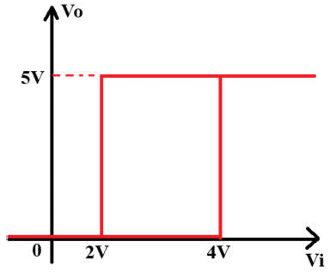
\includegraphics[width=\linewidth]{./my-chapters/my-images/Question11/debai_6a.png}
		\caption*{Hình 11a.}
		\label{fig:debai_11a}
	\end{figure}
\end{minipage}
\begin{minipage}{.5\linewidth}
	\begin{figure}[H]
		\centering
		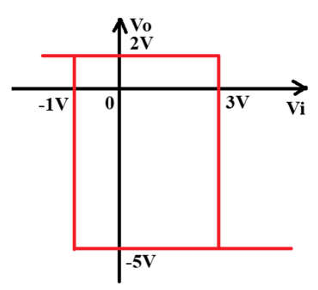
\includegraphics[width=\linewidth]{./my-chapters/my-images/Question11/debai_6b.png}
		\caption*{Hình 11b.}
		\label{fig:debai_11b}
	\end{figure}
\end{minipage}

\answer{a}{Mạch Schmitt Trigger không đảo.}

\begin{figure}[H]
	\centering
	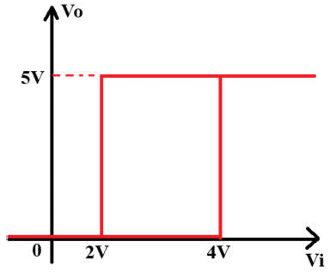
\includegraphics[width=.4\linewidth]{./my-chapters/my-images/Question11/debai_6a.png}
	\caption{Đồ Thị Mạch SMITCH TRIGGER không đảo.}
\end{figure}

Từ đồ thì ta có, $V_{UT} = 4\,\textsf{V}\text{; }V_{LT} = 2\,\textsf{V}$. Tương đương với với mạch SMITCH TRIGGER $V_{UT} = 1V ; V_{LT} = -1\,\textsf{V}$ và dời sang phải $3\textsf{V}$.

\begin{figure}[H]
	\centering
	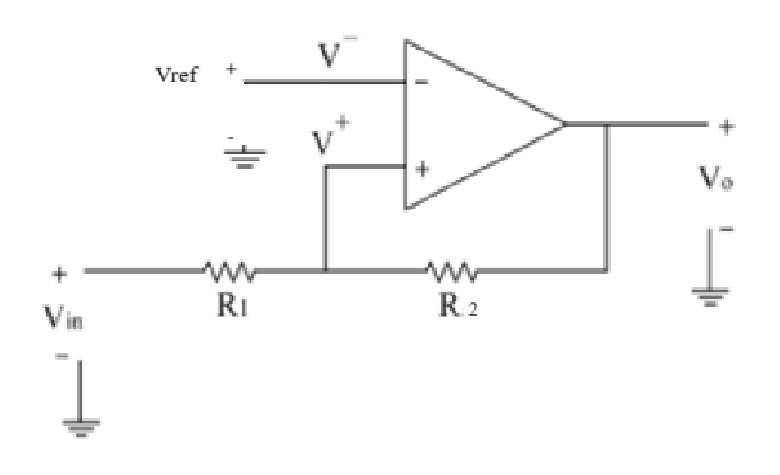
\includegraphics[width=.9\linewidth]{./my-chapters/my-images/Question11/C11_Hình2.png}
	\caption{SMITCH TRIGGER  không đảo.}
\end{figure}

\[V^+ > V^- = V_{ref} \rightarrow V_o = V_H = 5\,\textsf{V}\]
\[V^+ < V^- = V_{ref} \rightarrow V_o = V_L = 0\,\textsf{V}\]
Ta có: $\quad \dfrac{V^+ - V_{in}}{R_1} + \dfrac{V^+ - V_o}{R_2} = 0$ 
$\rightarrow V^+ = \dfrac{R_2}{R_1 + R_2}V_{in} + \dfrac{R_1}{R_1 + R_2}V_o$

Khi $V_o$ đang ở mức thấp để mạch chuyển sang mức cao: \\
$\rightarrow V^+ > V_{ref} \rightarrow \dfrac{R_2}{R_1 + R_2}V_{in} + \dfrac{R_1}{R_1 + R_2}V_o > V_{ref} $ \\[6pt]
$\rightarrow V_{in} > \dfrac{-R_1}{R_2}V_L + V_{ref}\dfrac{R_2 + R_1}{R_2}$ \\[4pt]
%$\rightarrow V_{in} > \dfrac{-R_1}{R_2}V_L + V_{ref}\dfrac{R_2 + R_1}{R_2}$ 
$\rightarrow V_{in} > V_{ref}\dfrac{R_2 + R_1}{R_2} = 4 \quad (1)$ \\[8pt]

Khi $V_o$ đang ở mức cao để mạch chuyển sang mức thấp: \\
$\rightarrow V^+ < V_{ref} \rightarrow$ 
$\dfrac{R_2}{R_1 + R_2}V_{in} + \dfrac{R_1}{R_1 + R_2}V_o < V_{ref} $ \\[6pt]
%$\rightarrow V_{in} < \dfrac{-R_1}{R_2}V_H + V_{ref}\dfrac{R_2 + R_1}{R_2}$ \\[6pt]
$\rightarrow V_{in} < -\dfrac{R_1}{R_2}V_H + V_{ref}\dfrac{R_2 + R_1}{R_2} $
$\rightarrow V_{in} < -\dfrac{R_1}{R_2}5 + V_{ref}\dfrac{R_2 + R_1}{R_2} = 2 \quad (2)$ \\[8pt]

Từ (1) và (2) $\rightarrow \dfrac{R_1}{R_2} = \dfrac{2}{5}$ \\[4pt]
Chọn \finalresult{R_1 = 2\,\textsf{k}\Omega}; \finalresult{R_2 = 5\,\textsf{k}\Omega}. 
$\rightarrow V_{ref} = 2.8571\,\textsf{V}$

\begin{figure}[H]
	\centering
	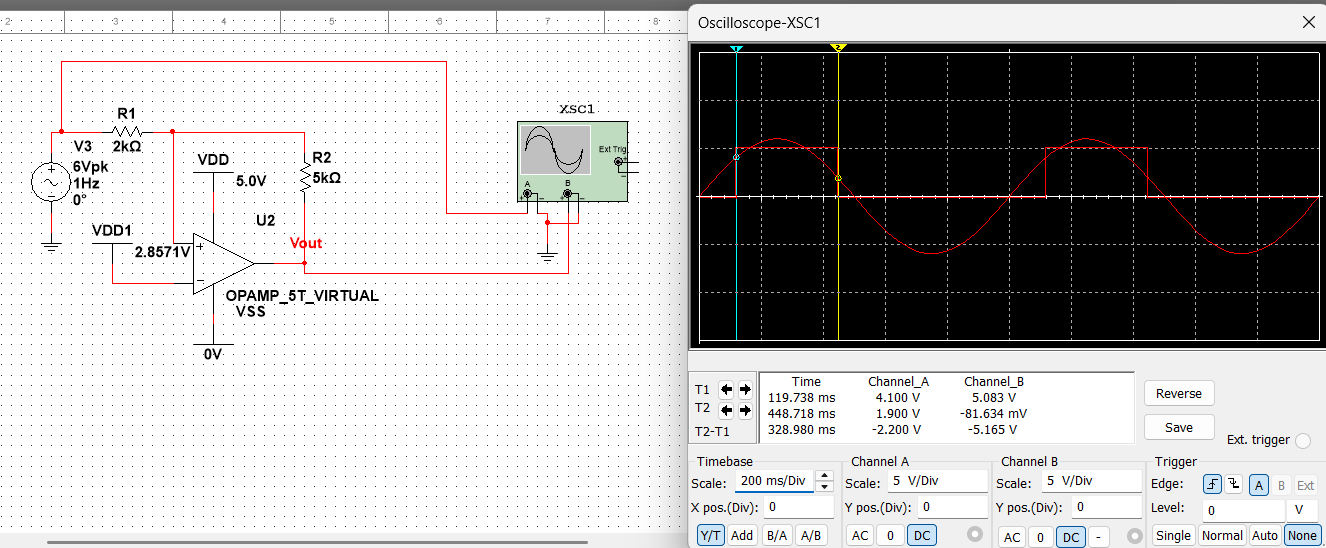
\includegraphics[width=.9\linewidth]{./my-chapters/my-images/Question11/C11_Hình3.png}
	\caption{Mô phỏng Multisim.}
\end{figure}

\answer{b}{Mạch Schmitt Trigger đảo.}

\begin{figure}[H]
	\centering
	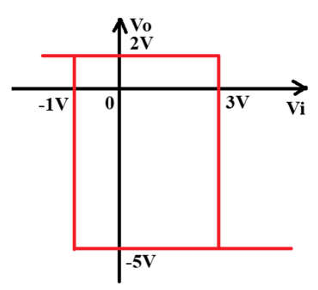
\includegraphics[width=.4\linewidth]{./my-chapters/my-images/Question11/debai_6b.png}
	\caption{Đồ Thị Mạch SMITCH TRIGGER đảo.}
\end{figure}

Từ đồ thì $\rightarrow V_{UT} = 3\,\textsf{V};\; V_{LT} = -1\,\textsf{V}$.

\begin{figure}[H]
	\centering
	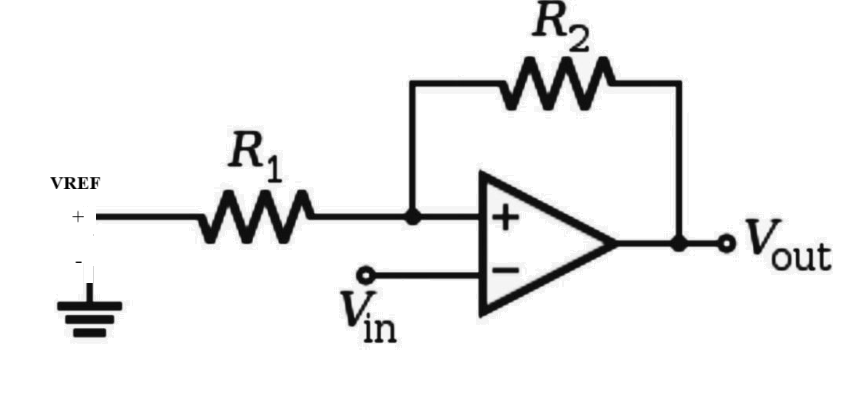
\includegraphics[width=.9\linewidth]{./my-chapters/my-images/Question11/C11_Hình5.png}
	\caption{SMITCH TRIGGER đảo.}
\end{figure}

\[
V^+ > V^- = V_{in} \rightarrow V_o = V_H = 2\,\textsf{V}
\]
\[
V^+ < V^- = V_{in} \rightarrow V_o = V_L = -5\,\textsf{V}
\]

Ta có: 
\[
\dfrac{V^+ - V_{ref}}{R_1} + \dfrac{V^+ - V_o}{R_2} = 0 
\rightarrow V^+ = \dfrac{R_2}{R_1 + R_2}V_{ref} + \dfrac{R_1}{R_1 + R_2}V_o
\]

Khi $V_o$ đang ở mức thấp để mạch chuyển sang mức cao: \\[4pt]
$\rightarrow V^+ > V_{in} \rightarrow 
\dfrac{R_2}{R_1 + R_2}V_{ref} + \dfrac{R_1}{R_1 + R_2}V_L > V_{in}$ \\[6pt]
$\rightarrow V_{in} < \dfrac{R_2}{R_1 + R_2}V_{ref} + \dfrac{R_1}{R_1 + R_2}V_L$ \\[4pt]
$\rightarrow V_{in} < \dfrac{R_2}{R_1 + R_2}V_{ref} - 5\,\dfrac{R_1}{R_1 + R_2} = -1 \quad (1)$ \\[8pt]

Khi $V_o$ đang ở mức cao để mạch chuyển sang mức thấp: \\[4pt]
$\rightarrow V^+ < V_{in} \rightarrow 
\dfrac{R_2}{R_1 + R_2}V_{ref} + \dfrac{R_1}{R_1 + R_2}V_o < V_{in}$ \\[6pt]
$\rightarrow V_{in} > \dfrac{R_2}{R_1 + R_2}V_{ref} + \dfrac{R_1}{R_1 + R_2}V_o$ \\[4pt]
$\rightarrow V_{in} > \dfrac{R_2}{R_1 + R_2}V_{ref} + \dfrac{R_1}{R_1 + R_2}\,2 = 3 \quad (2)$ \\[8pt]

Từ (1) và (2) $\rightarrow \dfrac{R_1}{R_2} = \dfrac{4}{3}$ \\[4pt]
Chọn \finalresult{R_1 = 4\,\textsf{k}\Omega}; \finalresult{R_2 = 3\,\textsf{k}\Omega}.
$\rightarrow V_{ref} = 4.33\,\textsf{V}$

\begin{figure}[H]
	\centering
	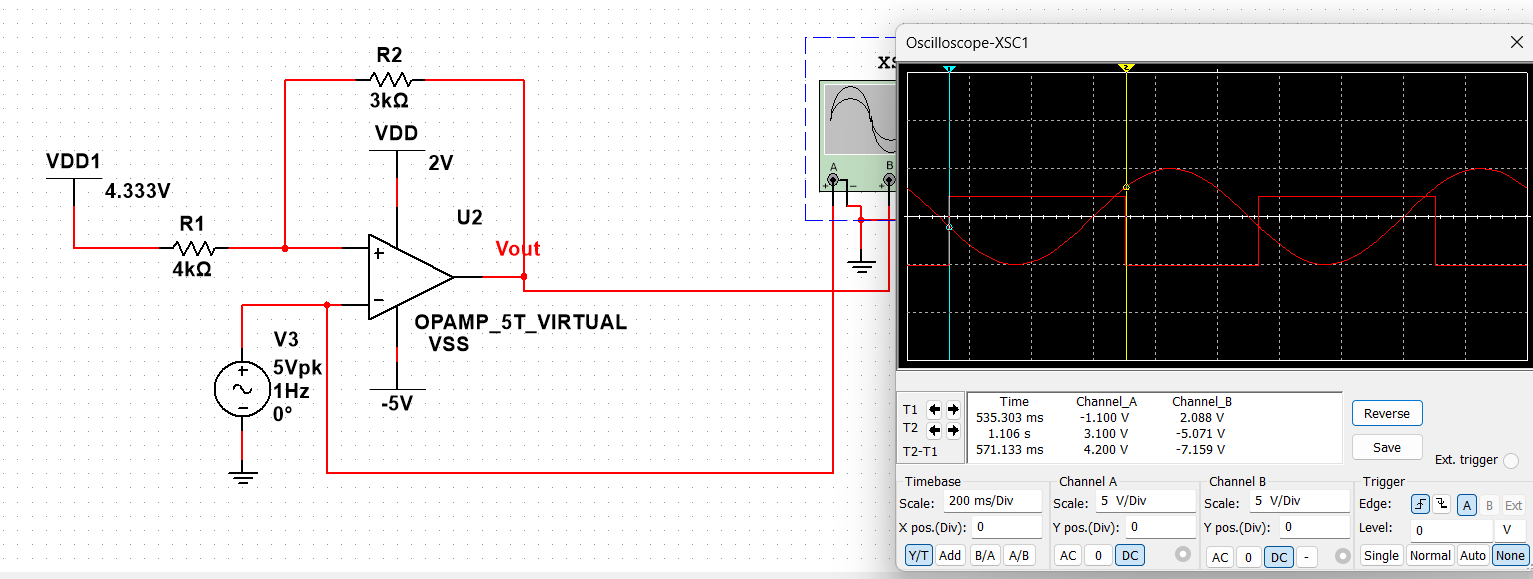
\includegraphics[width=.9\linewidth]{./my-chapters/my-images/Question11/C11_Hình6.png}
	\caption{Mô phỏng Multisim.}
\end{figure}